\documentclass[submit]{harvardml}

\course{CS181-S22}
\assignment{Assignment \#1}
\duedate{7:59pm ET, February 4, 2022} 

\usepackage[OT1]{fontenc}
\usepackage[colorlinks,citecolor=blue,urlcolor=blue]{hyperref}
\usepackage[pdftex]{graphicx}
\usepackage{graphicx}
\usepackage{caption}
\usepackage{fullpage}
\usepackage{soul}
\usepackage{amsmath}
\usepackage{amssymb}
\usepackage{color}
\usepackage{todonotes}
\usepackage{listings}
\usepackage{common}
\usepackage{framed}

\usepackage[mmddyyyy,hhmmss]{datetime}

\definecolor{verbgray}{gray}{0.9}

\lstnewenvironment{csv}{
  \lstset{backgroundcolor=\color{verbgray},
  frame=single,
  framerule=0pt,
  basicstyle=\ttfamily,
  columns=fullflexible}}{}
 

\begin{document}
\begin{center}
{\Large Homework 1: Regression}\\
\end{center}

\subsection*{Introduction}
This homework is on different forms of linear regression and focuses
on loss functions, optimizers, and regularization. Linear regression
will be one of the few models that we see that has an analytical
solution.  These problems focus on deriving these solutions and
exploring their properties.

If you find that you are having trouble with the first couple
problems, we recommend going over the fundamentals of linear algebra
and matrix calculus (see links on website).  The relevant parts of the
\href{https://github.com/harvard-ml-courses/cs181-textbook/blob/master/Textbook.pdf}{cs181-textbook notes are Sections 2.1 - 2.7}.  We strongly recommend
reading the textbook before beginning the homework.

    We also encourage you to first read the \href{http://users.isr.ist.utl.pt/~wurmd/Livros/school/Bishop\%20-\%20Pattern\%20Recognition\%20And\%20Machine\%20Learning\%20-\%20Springer\%20\%202006.pdf}{Bishop textbook}, particularly:
Section 2.3 (Properties of Gaussian Distributions), Section 3.1
(Linear Basis Regression), and Section 3.3 (Bayesian Linear
Regression). (Note that our notation is slightly different but the
underlying mathematics remains the same!).

\textbf{Please type your solutions after the corresponding problems using this
\LaTeX\ template, and start each problem on a new page.} You may find
the following introductory resources on \LaTeX\ useful: 
\href{http://www.mjdenny.com/workshops/LaTeX_Intro.pdf}{\LaTeX\ Basics} 
and \href{https://www.overleaf.com/learn/latex/Free_online_introduction_to_LaTeX_(part_1)}{\LaTeX\ tutorial with exercises in Overleaf}

Homeworks will be submitted through Gradescope. You will be added to
the course Gradescope once you join the course Canvas page. If you
haven't received an invitation, contact the course staff through Ed.

\textbf{Please submit the writeup PDF to the Gradescope assignment
  `HW1'.} Remember to assign pages for each question.

\textbf{Please submit your \LaTeX file and code files to the
  Gradescope assignment `HW1 - Supplemental'.} Your files should be
named in the same way as we provide them in the repository,
e.g. \texttt{T1\_P1.py}, etc.


%%%%%%%%%%%%%%%%%%%%%%%%%%%%%%%%%%%%%%%%%%%%%
% Problem 1
%%%%%%%%%%%%%%%%%%%%%%%%%%%%%%%%%%%%%%%%%%%%%

\begin{problem}[Optimizing a Kernel, 15pts]

Kernel-based regression techniques are similar to nearest-neighbor
regressors: rather than fit a parametric model, they predict values
for new data points by interpolating values from existing points in
the training set.  In this problem, we will consider a kernel-based
regressor of the form:
\begin{equation*}
  f(x^*) = \sum_{n} K(x_n,x^*) y_n 
\end{equation*}
where $(x_n,y_n)$ are the training data points, and $K(x,x')$ is a
kernel function that defines the similarity between two inputs $x$ and
$x'$. Assume that each $x_i$ is represented as a column vector, i.e. a
$D$ by 1 vector where $D$ is the number of features for each data
point. A popular choice of kernel is a function that decays as the
distance between the two points increases, such as
\begin{equation*}
  K(x,x') = \exp\left(\frac{-||x-x'||^2_2}{\tau}\right) = \exp\left(\frac{-(x-x')^T (x-x')}{\tau} \right) 
\end{equation*}
where $\tau$ represents the square of the lengthscale (a scalar value).  In this
problem, we will consider optimizing what that (squared) lengthscale
should be.

\begin{enumerate}

\item Let $\{(x_n,y_n)\}_{n=1}^N$ be our training data set.  Suppose
  we are interested in minimizing the residual sum of squares.  Write
  down this loss over the training data $\mcL(W)$ as a function of $\tau$.

  Important: When computing the prediction $f(x_i)$ for a point $x_i$
  in the training set, carefully consider for which points $x'$ you should be including
  the term $K(x_i,x')$ in the sum.

\item Take the derivative of the loss function with respect to $\tau$.
\end{enumerate}

\end{problem}

\newpage

\begin{framed}
\noindent\textbf{Problem 1} (cont.)\\

\begin{enumerate}
\setcounter{enumi}{2}
\item Consider the following data set:
\begin{csv}
  x , y
  0 , 0
  1 , 0.5
  2 , 1
  3 , 2
  4 , 1
  6 , 1.5
  8 , 0.5 
\end{csv}
And the following lengthscales: $\tau=.01$, $\tau=2$, and $\tau=100$.

Write some Python code to compute the loss with respect to each kernel
for the dataset provided above. Which lengthscale does best?  
For this problem, you can use our staff \textbf{script to compare your
  code to a set of staff-written test cases.} This requires, however,
that you use the structure of the starter code provided in
\texttt{T1\_P1.py}. More specific instructions can be found at the top
of the file \texttt{T1\_P1\_Testcases.py}. You may run the test cases
in the command-line using \texttt{python T1\_P1\_TestCases.py}.
\textbf{Note that our set of test cases is not comprehensive: just
  because you pass does not mean your solution is correct! We strongly
  encourage you to write your own test cases and read more about ours
  in the comments of the Python script.}
  
\item Plot the function $(x^*, f(x^*))$ for each of the
  lengthscales above.  You will plot $x^*$ on the x-axis and the
  prediction $f(x^*)$ on the y-axis.  For the test inputs $x^*$, you
  should use an even grid of spacing of $0.1$ between $x^* = 0$ and
  $x^* = 12$.  (Note: it is possible that a test input $x^*$ lands
  right on top of one of the training inputs above.  You can still use
  the formula!) 

  Initial impressions: Briefly describe what happens in each of the
  three cases.  Is what you see consistent with the which lengthscale
  appeared to be numerically best above?  Describe why or why not.

\item Bonus: Code up a gradient descent to optimize the kernel for the
  data set above.
  Start your gradient descent from $\tau=2$. Report on what you
  find.\\\\

  Note: Gradient descent is discussed in Section 3.4 of the
  cs181-textbook notes and Section 5.2.4 of Bishop, and will be
  covered later in the course!

\end{enumerate}
  
\end{framed}  

\newpage

\noindent\textbf{Solution 1.1:}\\
To find the loss over the training data, we find the squared difference between the $y_n$'s in the training data and the predicted values $\hat{y}_n = f(x_n)$:
\begin{align*}
    \mcL(W) &= \sum_{n=1}^{N} (y_n - f(x_n))^2\\
    \mcL(W) &= \sum_{n=1}^{N} (y_n - \sum_{i\ne n}^{N}K(x_i,x_n)y_i)^2\\
    \mcL(W) &= \sum_{n=1}^{N} (y_n - \sum_{i\ne n}^{N}\exp\left(\frac{-(x_i-x_n)^T (x_i-x_n)}{\tau} \right) y_i)^2
\end{align*}

\bigskip
\noindent\textbf{Solution 1.2:}\\
The derivative of the loss function with respect to $\tau$ is found by differentiating $\mcL(W)$ found in 1.1.
\begin{align*}
    \frac{d\mcL(W)}{d\tau} &= -2 \sum_{n=1}^{N} (y_n - \sum_{i\ne n}^{N} \exp\left(\frac{-(x_i-x_n)^T (x_i-x_n)}{\tau} \right) y_i) (\sum_{i\ne n}^{N} \frac{(x_i-x_n)^T (x_i-x_n)}{\tau^2} \exp\left(\frac{-(x_i-x_n)^T (x_i-x_n)}{\tau} \right) y_i)
\end{align*}

\bigskip
\noindent\textbf{Solution 1.3:}\\
Computing the loss with respect to each kernel (with different values of $\tau$) yields that $\tau = 2$ produces the lowest residual sum of squares, i.e. the least loss. Therefore, we can say that $\tau = 2$ is the lengthscale that does best with the dataset provided.
\begin{center}
\begin{tabular}{ |c|c|c| } 
 \hline
 $\tau$ & $\mcL(W)$ \\ 
 \hline\hline
 $0.01$ & $8.75$ \\
 \hline
 $2$ & $3.305016494565789$ \\ 
 \hline
 $100$ & $120.35919342230957$ \\ 
 \hline
\end{tabular}
\end{center}

\bigskip
\noindent\textbf{Solution 1.4:}\\
\begin{center}
    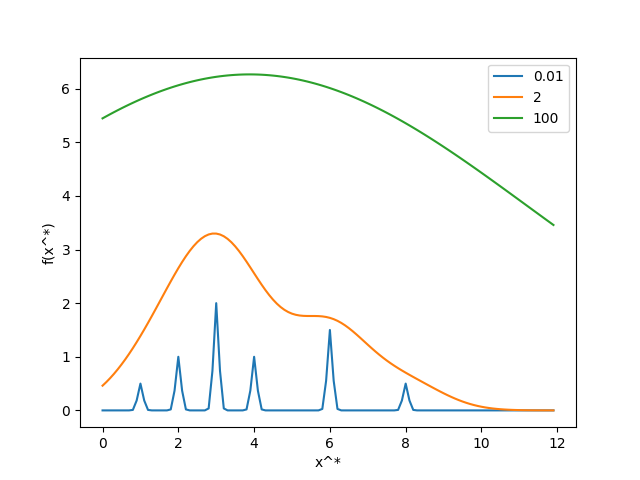
\includegraphics[scale=0.7]{1.4.png}
\end{center}
When $\tau = 0.01$, the model predicts the values of $y$ for points in training data almost perfectly, but offers practically no insight on what $y$ is at other values of $x$, defaulting to $y \approx 0$ at all other $x$ values. This occurs because, when $\tau$ is small, $K(x, x')$ tends towards $0$, unless $||x-x'||^2_2$ is close to $0$ (i.e. you have two very nearby points), in which case $K(x, x')$ tends towards $1$. Therefore, when predicting a point at an $x^*$ that is equal to an $x_i$ in the training data $K(x_i, x^*)$ tends towards $1$ and $K(x \ne x_i, x^*)$ tends towards $0$, so $f(x^*)$ tends towards $y_i$. Thus, when $\tau = 0.01$, the model greatly overfits the training data and is not generalizable, even though it had the second best loss metric.\\

\noindent When $\tau = 2$, the model produces a smooth curve over a set of $y$ values that closely (albeit not perfectly) predict the points occurring in the testing data, giving this model a low loss and better generalizability. It also predicts $y$ values that are too large because we did not normalize for the weights given to the $y$ points used to predict $f(x^*)$ (see further explanation of this below when $\tau = 100$).\\

\noindent When $\tau = 100$, the model produces an even simpler smooth curve over a set of $y$ values that predict the points occurring in the testing data less well than the previous models, i.e. underfitting the training data. It also predicts $y$ values that are too large. This occurs because $\tau$ is effectively acting as a regularization parameter, penalizing large weights that are given to $y$'s corresponding to $x$'s that are close to $x^*$, and giving more weight (in comparison to previous models) to $y$'s corresponding to $x$'s that are further away from this $x^*$. Furthermore, in this model we did not normalize for the weights given to the $y$ points used to predict $f(x^*)$, so when the weight given to $x$'s that are further away from $x^*$ do not decay to $0$, the model ends up overestimating $f(x^*)$. Given the curve produced by this model is less expressive, it also makes it worse at interpolating and extrapolating from the training data, so ends up having the highest loss.\\

\newpage

%%%%%%%%%%%%%%%%%%%%%%%%%%%%%%%%%%%%%%%%%%%%%
% Problem 2
%%%%%%%%%%%%%%%%%%%%%%%%%%%%%%%%%%%%%%%%%%%%%

\begin{problem}[Kernels and kNN, 10pts]

Now, let us compare the kernel-based approach to an approach based on
nearest-neighbors.  Recall that kNN uses a predictor of the form
  \begin{equation*}
    f(x^*) = \frac{1}{k} \sum_n y_n \mathbb{I}(x_n \texttt{ is one of k-closest to } x^*)
  \end{equation*}

\noindent where $\mathbb{I}$ is an indicator variable. For this problem, you will use the \textbf{same dataset and kernel as in Problem 1}.


For this problem, you can use our staff \textbf{script to compare your code to a set of staff-written test cases.} This requires, however, that you use the structure of the starter code provided in \texttt{T1\_P2.py}. More specific instructions can be found at the top of the file \texttt{T1\_P2\_Testcases.py}. You may run the test cases in the command-line using \texttt{python T1\_P2\_TestCases.py}.
\textbf{Note that our set of test cases is not comprehensive: just because you pass does not mean your solution is correct! We strongly encourage you to write your own test cases and read more about ours in the comments of the Python script.}

\vspace{0.5cm}
\noindent\emph{Make sure to include all required plots in your PDF.}


\begin{enumerate}

\item Implement kNN for $k=\{1, 3, N-1\}$ where N is the size of the dataset, then plot the results for each $k$. To find the distance between points, use the kernel function from Problem 1 with lengthscale $\tau=1$. 

As before, you will plot $x^*$ on the x-axis and the prediction $f(x^*)$ on the y-axis.  For the test inputs $x^*$, you should use an even grid of spacing of $0.1$ between $x^* = 0$ and $x^* = 12$.  (Like in Problem 1, if a test point lies on top of a training input, use the formula without excluding that training input.)
  
  You may choose to use some starter Python code to create your plots
  provided in \verb|T1_P2.py|.  Please \textbf{write your own
    implementation of kNN} for full credit.  Do not use external
  libraries to find nearest neighbors.
  
\item Describe what you see: What is the behavior of the functions in
  these three plots?  How does it compare to the behavior of the
  functions in the three plots from Problem 1?  Are there situations
  in which kNN and kernel-based regression interpolate similarly?
  Extrapolate similarly?  Based on what you see, do you believe there
  exist some values of $k$ and $\tau$ for which the kNN and kernel-based regressors produce the exact same classifier (ie. given \textit{any} point $x$, the two regressors will produce the same prediction $f(x)$)? Explain your answer.
  
\item Why did we not vary $\tau$ for the kNN approach?

\end{enumerate}

\end{problem}

\newpage

\noindent\textbf{Solution 2.1:}\\
\begin{center}
    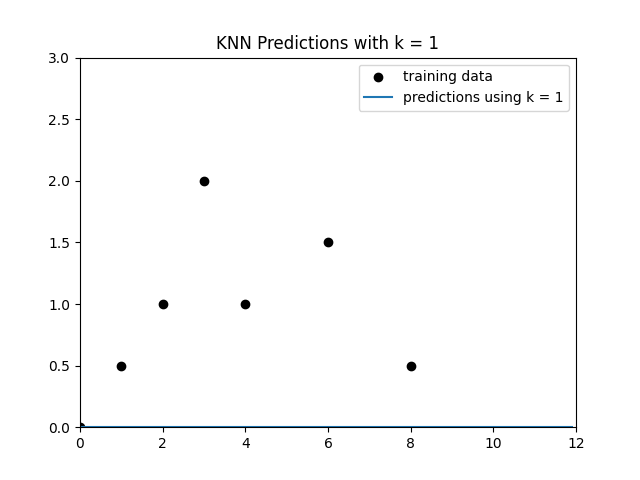
\includegraphics[scale=0.5]{k1.png}
\end{center}
\begin{center}
    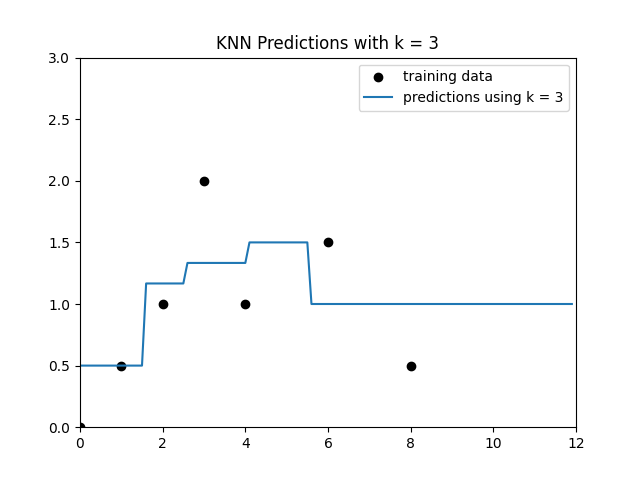
\includegraphics[scale=0.5]{k3.png}
\end{center}
\begin{center}
    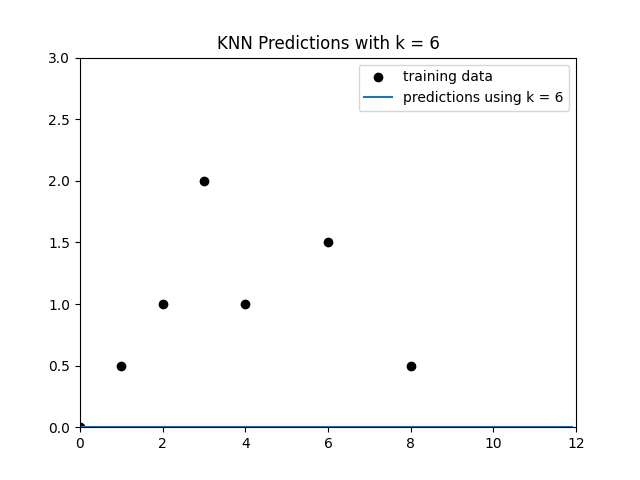
\includegraphics[scale=0.5]{k6.png}
\end{center}
\newpage

\noindent\textbf{Solution 2.2:}\\
When $k = 1$, the model predicts the values of $y$ for points in training data perfectly, but clearly is overfitting to these data. This makes sense conceptually, as this model is finding the nearest (measured by the kernel) $x_i$ in the training data to $x^*$ and taking the corresponding $y_i$ to be $f(x^*)$. For all $x_i$ where $i \ne 0, N$, this $y_i$ is given to be the predicted value for all $x$ inputs on the range $[\frac{x_{n} + x_{n-1}}{2}, \frac{x_{n} + x_{n+1}}{2})$. Hence, we get what looks what a piecewise function that perfectly fits the training data. This is certainly similar to the plot with $\tau = 0.01$ from Problem 1, in terms of overfitting the training data.\\

\noindent When $k = 3$, the model predicts the values of $y$ for points in training data slightly less well, and is not overfitting to these data as much. This makes sense conceptually, as this model is finding the nearest (measured by the kernel) 3 $x_i$'s in the training data to $x^*$ and taking the average of the corresponding 3 $y_i$'s to be $f(x^*)$. This has a similar behaviour to the plot with $\tau = 2$ from Problem 1, in terms of producing a middle-ground between $k=1$ and $k=N-1$ - neither overtly overfitting nor underfitting to the training data.\\

\noindent When $k = N-1$, the model produces what looks like a piecewise function with two pieces: for $x^*<4$, $f(x^*)$ is the average of the $y_i$'s corresponding to $x_0, ..., x_{N-1}$; for $x^*>4$, $f(x^*)$ is the average of the $y_i$'s corresponding to $x_1, ..., x_N$. This has a similar behaviour to the plot with $\tau = 100$ from Problem 1, in terms of producing a line that is less expressive than the other models', and so underfits the data.\\

\noindent Given the behaviour of these plots is similar to the respective plots from Problem 1, it can be said that they interpolate similarly. However, they extrapolate quite differently. Since, kNN regressors produce what look like piecewise functions, for $x^*>x_N$, $f(x^*)=f(x_N)$, and the kNN regressors give no additional information when extrapolating outside of the domain of the data. By comparison, kernel-based regressors have some additional predictive power when extrapolating; since they generate smooth curves (when $\tau$ is sufficiently greater than $0.01$), for $x^*>x_N$, $f(x^*) \ne f(x_N)$. Given such differences between the geometry of the plots, kNN and kernel-based regressors will not produce the exact same classifier (i.e. $f(x^*)$) for a given $x^*$.

\bigskip
\noindent\textbf{Solution 2.3:}\\
Given $\tau$ is a positive scalar, it simply re-scales the distances between $x^*$ and its nearest neighbors but has no effect on the ranking of $x^*$'s nearest neighbors. This means that if $x_1$ is nearer to $x^*$ than $x_2$ with $\tau$ equal to some $c$ (where $c \in \mathbb{R}^{+}$), $x_1$ is nearer to $x^*$ than $x_2$ for all possible values of $c$. Thus, varying $\tau$ would have no effect on the $y_n$'s which we average to get $f(x^*)$, so we do not bother varying $\tau$ for the kNN approach.

\newpage 

%%%%%%%%%%%%%%%%%%%%%%%%%%%%%%%%%%%%%%%%%%%%%
% Problem 3
%%%%%%%%%%%%%%%%%%%%%%%%%%%%%%%%%%%%%%%%%%%%%

\begin{problem}[Deriving Linear Regression, 10pts]

  The solution for the least squares linear regressions ``looks'' kind
  of like a ratio of covariance and variance terms.  In this problem,
  we will make that connection more explicit. \\

  \noindent Let us assume that our data are tuples of scalars $(x,y)$ that are
  described by some joint distribution $p(x,y)$.  For clarification, the joint distribution $p(x,y)$ is just another way of saying the ``joint PDF'' $f(x,y)$, which may be more familiar to those who have taken Stat 110, or equivalent. \\
  
  \noindent We will consider the process of fitting these data from this distribution with the best linear model
  possible, that is a linear model of the form $\hat{y} = wx$ that
  minimizes the expected squared loss $E_{x,y}[ ( y - \hat{y} )^2
  ]$.\\

\noindent \emph{Notes:} The notation $E_{x, y}$ indicates an
expectation taken over the joint distribution $p(x,y)$.  Since $x$ and
$y$ are scalars, $w$ is also a scalar.
  
  \begin{enumerate}

  \item Derive an expression for the optimal $w$, that is, the $w$
    that minimizes the expected squared loss above.  You should leave
    your answer in terms of moments of the distribution, e.g. terms
    like $E_x[x]$, $E_x[x^2]$, $E_y[y]$, $E_y[y^2]$, $E_{x,y}[xy]$
    etc.

\item Provide unbiased and consistent formulas to estimate $E_{x, y}[yx]$
 and $E_x[x^2]$ given observed data $\{(x_n,y_n)\}_{n=1}^N$.

\item In general, moment terms like $E_{x, y}[yx]$, $E_{x, y}[x^2]$,
  $E_{x, y}[yx^3]$, $E_{x, y}[\frac{x}{y}]$, etc. can easily be
  estimated from the data (like you did above).  If you substitute in
  these empirical moments, how does your expression for the optimal
  $w^*$ in this problem compare with the optimal $w^*$ that we see in
  Section 2.6 of the cs181-textbook?

\item Many common probabilistic linear regression models assume that
  variables x and y are jointly Gaussian.  Did any of your above
  derivations rely on the assumption that x and y are jointly
  Gaussian?  Why or why not?
    
\end{enumerate}

\end{problem}

\newpage

\noindent\textbf{Solution 3.1:}\\
In this problem, we are given that the linear model has the form $\hat{y} = wx$. Substituting this into the expected squared loss gives:
\begin{align*}
    E_{x,y}[ ( y - \hat{y} )^2] &= E_{x,y}[ ( y - wx )^2]   
\end{align*}
Expanding the brackets and applying linearity of expectation gives:
\begin{align*}
    E_{x,y}[ ( y - \hat{y} )^2] &= E_{x,y}[ y^2 - 2wxy + w^2 x^2]\\
    &= E_{x,y}[ y^2 ] - 2wE_{x,y}[xy] + w^2 E_{x,y}[x^2]
\end{align*}
We can drop the $y$ subscript for expectations involving only $x$ and the $x$ subscript for expectations involving only $y$:
\begin{align*}
    E_{x,y}[ ( y - \hat{y} )^2] &= E_{y}[ y^2 ] - 2wE_{x,y}[xy] + w^2 E_{x}[x^2]
\end{align*}
To find the optimal $w$ that minimizes the expected square loss above, we take the derivative of this expression with respect to $w$, set equal to 0, and solve for $w$:
\begin{align*}
    \frac{d}{dw} [ E_{y}[ y^2 ] - 2wE_{x,y}[xy] + w^2 E_{x}[x^2] ] &= 0\\
    \implies - 2E_{x,y}[xy] + 2w E_{x}[x^2] &= 0\\
    \implies w = \frac{E_{x,y}[xy]}{E_{x}[x^2]}
\end{align*}

\bigskip
\noindent\textbf{Solution 3.2:}\\
Unbiased and consistent formulas that estimate these expectations can be found using the Law of Large Numbers which states that for large data sets a sample mean $\Bar{X}_n$ converges to the true mean pointwise, with probability 1, i.e. $P(\Bar{X}_n \rightarrow \mu) = 1$. Thus, given observed data $\{(x_n,y_n)\}_{n=1}^N$, assuming $N$ is sufficiently large:
\begin{align*}
    E_{x,y}[xy] &= \frac{1}{N} \sum_{n=1}^{N} x_n y_n \text{ with probability } 1\\
    E_{x}[x^2] &= \frac{1}{N} \sum_{n=1}^{N} x_n^2 \text{ with probability } 1
\end{align*}

\bigskip
\noindent\textbf{Solution 3.3:}\\
Substituting in these moment terms from 3.2 into the expression for the optimal $w$ from 3.1 gives:
\begin{align*}
    w^* &= \frac{\frac{1}{N} \sum_{n=1}^{N} x_n y_n}{\frac{1}{N} \sum_{n=1}^{N} x_n^2}\\
    &= \frac{\sum_{n=1}^{N} x_n y_n}{\sum_{n=1}^{N} x_n^2}
\end{align*}

\noindent This expression is the 1-dimensional version of the Moore-Penrose pseudo inverse seen in section 2.6 of the textbook, $(\mathbf{X}^\top \mathbf{X})^{-1} \mathbf{X}^\top \mathbf{y}$. $\mathbf{X}$ is a Nx1 vector containing all the $x_i$'s, so $(\mathbf{X}^\top \mathbf{X})^{-1}$ is the inverse/reciprocal of a scalar equal to $\frac{1}{\sum_{n=1}^{N} x_n^2}$. Likewise $\mathbf{y}$ is a Nx1 vector containing all the $y_i$'s, so $\mathbf{X}^\top \mathbf{y}$ is equal to the scalar $\sum_{n=1}^{N} x_n y_n$. Thus, in the 1-dimensional case, where $\mathbf{X}$ and $\mathbf{y}$ are Nx1 vectors, $w^*$ is given by the expression above.

\bigskip
\noindent\textbf{Solution 3.4:}\\
No. None of the steps in the derivations above (linearity of expectation, differentiation, Law of Large Numbers) relied on an assumption that variables $x$ and $y$ are jointly Gaussian. Furthermore, the cs181-textbook shows that solving for $w^*$ by minimizing the loss function, as we did in this problem, is equivalent to maximizing the probability under the assumption of a linear model with Gaussian noise. Thus, we can clearly use this process for models in which $x$ and $y$ are not jointly Gaussian.


%%%%%%%%%%%%%%%%%%%%%%%%%%%%%%%%%%%%%%%%%%%%%
% Problem 4
%%%%%%%%%%%%%%%%%%%%%%%%%%%%%%%%%%%%%%%%%%%%%

\begin{problem}[Modeling Changes in Republicans and Sunspots, 15pts]
  
 The objective of this problem is to learn about linear regression
 with basis functions by modeling the number of Republicans in the
 Senate. The file \verb|data/year-sunspots-republicans.csv| contains the
 data you will use for this problem.  It has three columns.  The first
 one is an integer that indicates the year.  The second is the number
 of Sunspots observed in that year.  The third is the number of Republicans in the Senate for that year.
 The data file looks like this:
 \begin{csv}
Year,Sunspot_Count,Republican_Count
1960,112.3,36
1962,37.6,34
1964,10.2,32
1966,47.0,36
\end{csv}

You can see scatterplots of the data in the figures below.  The horizontal axis is the Year, and the vertical axis is the Number of Republicans and the Number of Sunspots, respectively.

\begin{center}
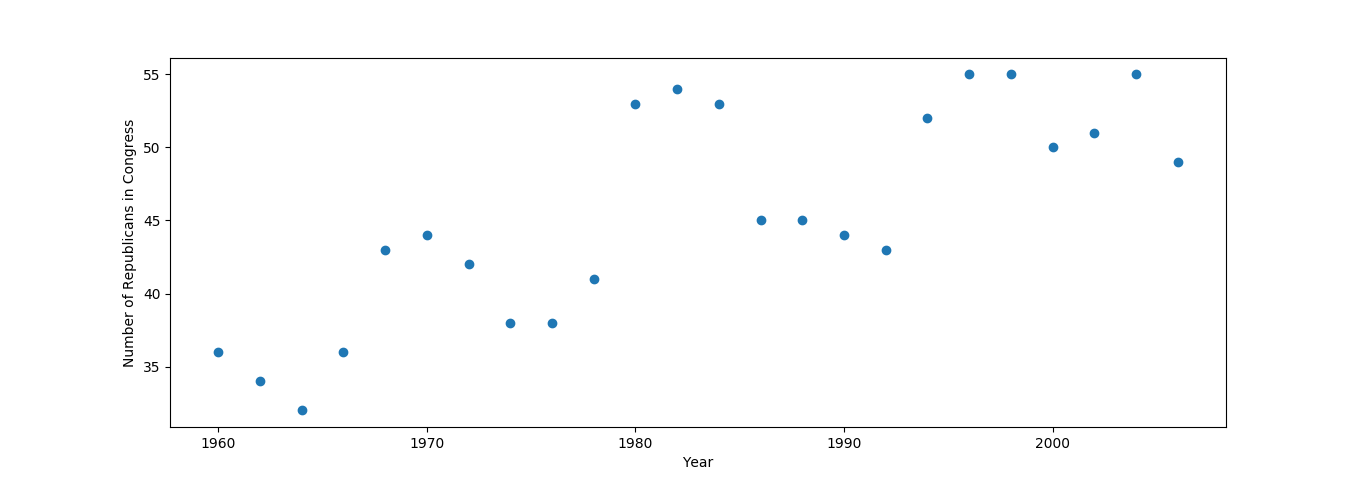
\includegraphics[width=.5\textwidth]{data/year-republicans}
\end{center}

\begin{center}
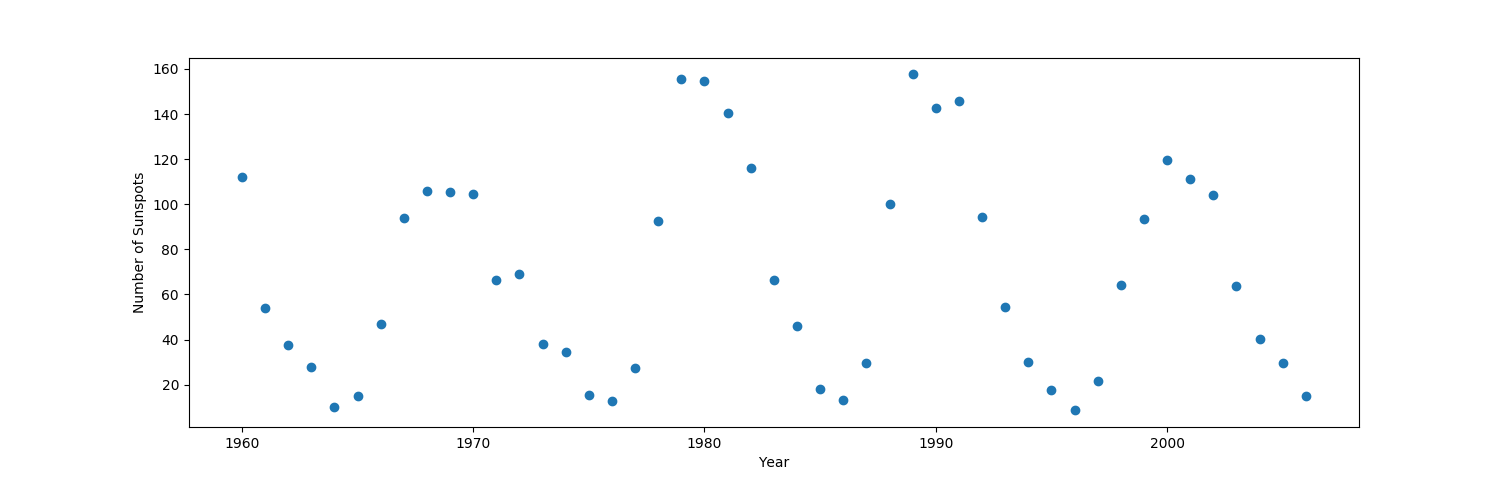
\includegraphics[width=.5\textwidth]{data/year-sunspots}
\end{center}

(Data Source: \url{http://www.realclimate.org/data/senators_sunspots.txt})\\
\vspace{-5mm}


\vspace{0.5cm}
\noindent\emph{Make sure to include all required plots in your PDF.}

\begin{enumerate}

\item In this problem you will implement ordinary least squares
  regression using 4 different basis functions for \textbf{Year
    (x-axis)} v. \textbf{Number of Republicans in the Senate
    (y-axis)}. Some starter Python code that implements simple linear
  regression is provided in \verb|T1_P4.py|.

  Note: The numbers in the \emph{Year} column are large (between $1960$ and $2006$), especially when raised to various powers. To avoid numerical instability due to ill-conditioned matrices in most numerical computing systems, we will scale the data first: specifically, we will scale all ``year'' inputs by subtracting $1960$ and then dividing by $40$. Similarly, to avoid numerical instability with numbers in the \emph{Sunspot\_Count} column, we will also scale the data first by dividing all ``sunspot count'' inputs by $20$. Both of these scaling procedures have already been implemented in lines $65-69$ of the starter code in \verb|T1_P4.py|. Please do \emph{not} change these lines!

First, plot the data and regression lines for each of the following sets of basis functions, and include
the generated plot as an image in your submission PDF. You will therefore make 4 total plots:
\begin{enumerate}
	\item[(a)] $\phi_j(x) = x^j$ for $j=1, \ldots, 5$\\
    ie, use basis $y = a_1 x^1 + a_2 x^2 + a_3 x^3 + a_4 x^4 + a_5 x^5$ for some constants $\{a_1, ..., a_5\}$. 
    \item[(b)] $\phi_j(x) = \exp{\frac{-(x-\mu_j)^2}{25}}$ for $\mu_j=1960, 1965, 1970, 1975, \ldots 2010$
	\item[(c)] $\phi_j(x) = \cos(x / j)$ for $j=1, \ldots, 5$
	\item[(d)] $\phi_j(x) = \cos(x / j)$ for $j=1, \ldots, 25$
\end{enumerate}
\vspace{-2mm}


{\footnotesize * Note: Please make sure to add a bias term for all your basis functions above in your implementation of the \verb|make_basis| function in \verb|T1_P4.py|.}
  
Second, for each plot include the residual sum of squares error. Submit the generated plot and residual sum-of-squares error for each basis in your LaTeX write-up.
\end{enumerate}

\end{problem}

\begin{framed}
\noindent\textbf{Problem 4} (cont.)\\
\begin{enumerate}
\setcounter{enumi}{1}
\item Repeat the same exact process as above but for \textbf{Number of Sunspots (x-axis)} v. \textbf{Number of Republicans in the Senate (y-axis)}. 
Now, however, only use data from before 1985, and only use basis functions (a), (c), and (d) -- ignore basis (b). You will therefore make 3 total plots. For each plot make sure to also include the residual sum of squares error.



Which of the three bases (a, c, d) provided the "best" fit? \textbf{Choose one}, and keep in mind the generalizability of the model. 

Given the quality of this fit, do you believe that the number of sunspots controls the number of Republicans in the senate (Yes or No)?
\end{enumerate}
\end{framed}

\newpage

\noindent\textbf{Solution 4.1:}\\
(a)
\begin{center}
    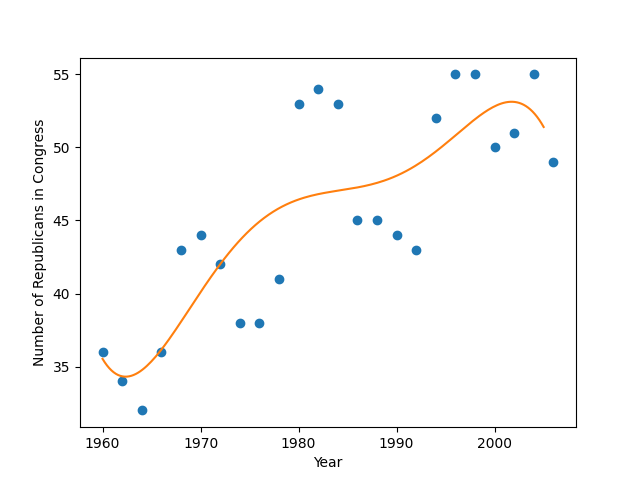
\includegraphics[scale=0.5]{4.1a.png}
\end{center}
(b)
\begin{center}
    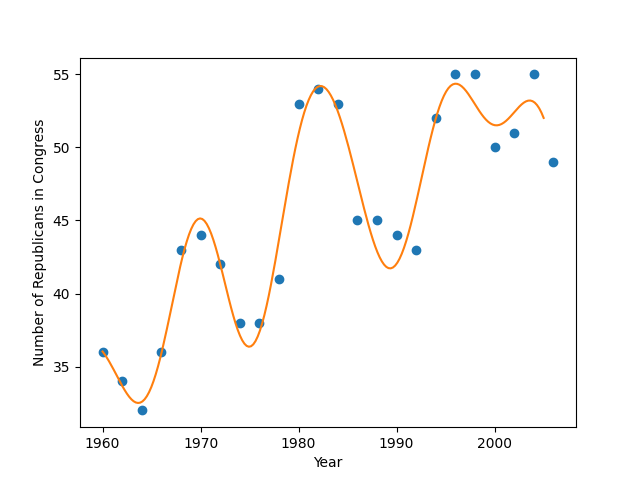
\includegraphics[scale=0.5]{4.1b.png}
\end{center}
(c)
\begin{center}
    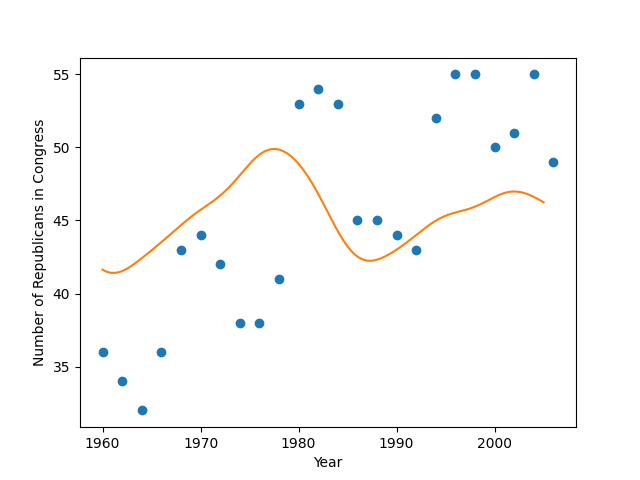
\includegraphics[scale=0.5]{4.1c.png}
\end{center}
(d)
\begin{center}
    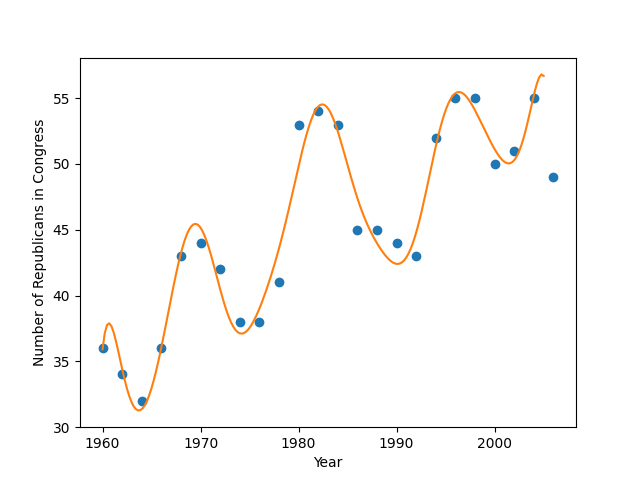
\includegraphics[scale=0.5]{4.1d.png}
\end{center}

\smallskip
\begin{center}
\begin{tabular}{ |c|c|c| } 
 \hline
 Basis & Residual sum of squares error \\ 
 \hline\hline
 (a) & $394.9803839890881$ \\
 \hline
 (b) & $54.27309661671943$ \\ 
 \hline
 (c) & $1082.8088559867188$ \\ 
 \hline
 (d) & $39.00107715663492$ \\ 
 \hline
\end{tabular}
\end{center}

\bigskip
\noindent\textbf{Solution 4.2:}\\
(a)
\begin{center}
    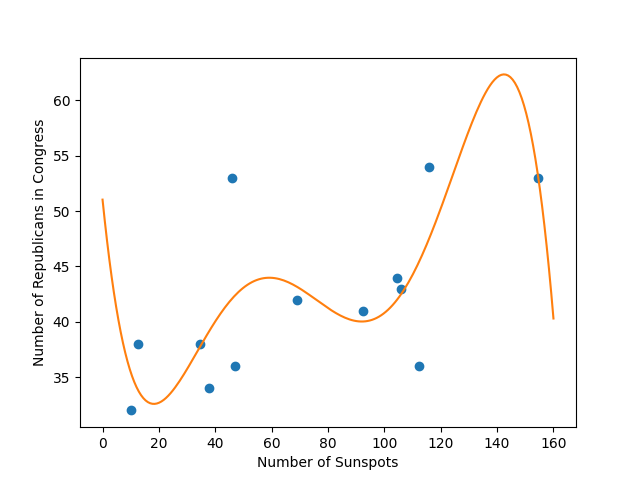
\includegraphics[scale=0.5]{4.2a.png}
\end{center}
(c)
\begin{center}
    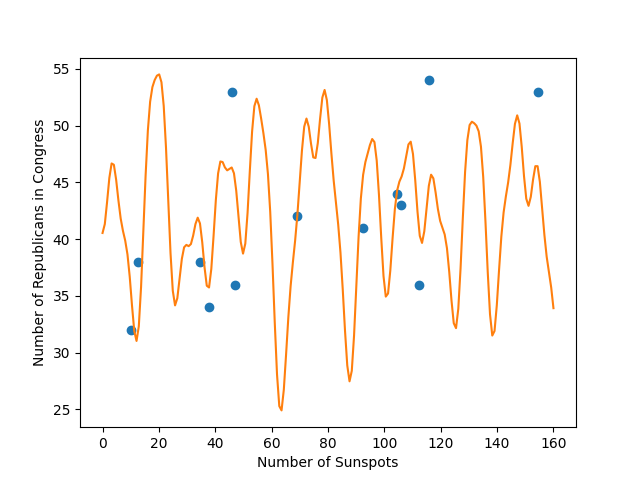
\includegraphics[scale=0.5]{4.2c.png}
\end{center}
(d)
\begin{center}
    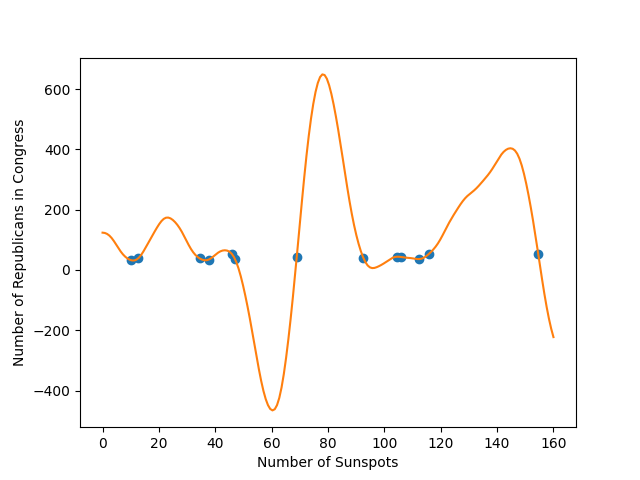
\includegraphics[scale=0.5]{4.2d.png}
\end{center}

\smallskip
\begin{center}
\begin{tabular}{ |c|c|c| } 
 \hline
 Basis & Residual sum of squares error \\ 
 \hline\hline
 (a) & $351.2279357741859$ \\
 \hline
 (c) & $375.10675778167405$ \\ 
 \hline
 (d) & $2.186325095811903 \times 10^{-22}$ \\ 
 \hline
\end{tabular}
\end{center}

\smallskip
\noindent Basis (d) provided the "best" fit for the training data in terms of least squares loss, but this is not necessarily easily generalizable given how it seems to overfit these data. Therefore, (a) seems more generalizable and can be argued to provide the "best" fit.\\

\noindent Even though basis (d) fit the data very well, simple logic tells is that the number of sunspots does not control the number of Republicans in the senate. This is an example of the old adage that "correlation does not equal causation"; in other words, regression can tell us that there is an association between two variables, but we cannot necessarily infer causality. Thus, even though we can make a model that fits the training data, it does not mean that sunspots control number of republicans.

\newpage
%%%%%%%%%%%%%%%%%%%%%%%%%%%%%%%%%%%%%%%%%%%%%
% Name and Calibration
%%%%%%%%%%%%%%%%%%%%%%%%%%%%%%%%%%%%%%%%%%%%%
\subsection*{Name}
Ben Ray

\subsection*{Collaborators and Resources}
Whom did you work with, and did you use any resources beyond cs181-textbook and your notes?\\
\smallskip
Worked with Elias Nuwara\\
Skyler's Code Review notes and Stack Overflow for help with Python syntax\\
CS 181 Office hours

\subsection*{Calibration}
Approximately how long did this homework take you to complete (in hours)?\\
\smallskip
20

\end{document}